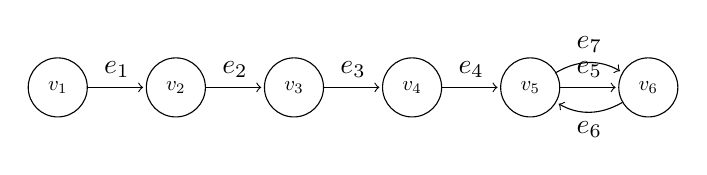
\begin{tikzpicture}[shorten >=1pt,node distance=2cm,auto,scale=1.5,nd/.style={draw=black,circle,scale=\sc,minimum width=0.75 cm,minimum height=1 cm},ndg/.style={nd,fill=gray}]
\def\sc{0.75}
\foreach \i in {1,...,6} {
  \node[nd] (v\i) at (\i,0) {$v_\i$};
}
\foreach \i/\j in {1/2,2/3,3/4,4/5,5/6} {
  \path[->] (v\i) edge node[midway,above] {$e_{\i}$} (v\j);
}
\path[->] (v6) edge[bend left] node[midway,below]{$e_6$} (v5);
\path[->] (v5) edge[bend left] node[midway,above]{$e_7$} (v6);
\end{tikzpicture}